\documentclass[french,11pt]{beamer}

\DeclareMathOperator{\Cov}{Cov}
\DeclareMathOperator{\Var}{Var}
\DeclareMathOperator{\E}{\mathbb{E}}
\DeclareMathOperator{\Proba}{\mathbb{P}}

\newcommand{\Covb}[2]{\ensuremath{\Cov\!\left[#1,#2\right]}}
\newcommand{\Eb}[1]{\ensuremath{\E\!\left[#1\right]}}
\newcommand{\Pb}[1]{\ensuremath{\Proba\!\left[#1\right]}}
\newcommand{\Varb}[1]{\ensuremath{\Var\!\left[#1\right]}}

% norm
\newcommand{\norm}[1]{\| #1 \|}

\newcommand{\indep}{\rotatebox[origin=c]{90}{$\models$}}





\usepackage{mathptmx,amsmath,amssymb,graphicx,bibentry,bbm,babel,ragged2e}

\makeatletter

\newcommand{\noun}[1]{\textsc{#1}}
\newcommand{\jitem}[1]{\item \begin{justify} #1 \end{justify} \vfill{}}
\newcommand{\sframe}[2]{\frame{\frametitle{#1} #2}}

\newenvironment{centercolumns}{\begin{columns}[c]}{\end{columns}}
%\newenvironment{jitem}{\begin{justify}\begin{itemize}}{\end{itemize}\end{justify}}

\usetheme{Warsaw}
\setbeamertemplate{footline}[text line]{}
\setbeamercolor{structure}{fg=purple!50!blue, bg=purple!50!blue}

\setbeamersize{text margin left=15pt,text margin right=15pt}

\setbeamercovered{transparent}


\@ifundefined{showcaptionsetup}{}{%
 \PassOptionsToPackage{caption=false}{subfig}}
\usepackage{subfig}

\usepackage[utf8]{inputenc}
\usepackage[T1]{fontenc}



\makeatother

\begin{document}


\title{For a Cautious Use of Big Data and Computation}

\author{J.~Raimbault$^{1,2}$\\
\texttt{juste.raimbault@parisgeo.cnrs.fr}
}


\institute{$^{1}$UMR CNRS 8504 G{\'e}ographie-cit{\'e}s\\
$^{2}$UMR-T IFSTTAR 9403 LVMT\\
}


\date{RGS 2016\\\smallskip
\textit{Session Geocomputation : The Next 20 years}\\\smallskip
September 2016
}

\frame{\maketitle}







%%%%%%%%%%%%%%%%
%%
%% IDEAS
%%
%%  -> ex of synthetic data - interpolation, extrapolation.
%%  -> ex of Pok.Go (cf geotamtam mail) : direct on data without thinking ?
%%  -> Claims : make a stronger link between computational practices and maths/stats ? (if possible) - need more interdisciplinarity to do that.
%%     Geography in the center of that dynamic, but not all for granted ! (eg not simulate Gibrat as the fool example !)
%%     It implies the need for elaborated theory : here trash West/Bettencourt.
%%  -> Mention Cybergeo/CybergeoNetworks
%%
%%  - example with journal/paper title : what ?



%%%%%%%%%
%% Abstract

%\textbf{Keywords : }\textit{Data Deluge, Computational Science, City-transportation Interactions, Spatio-temporal Correlations}

%The so-called \emph{big data revolution} resides as much in the availability of large datasets of novel and various types as in the always increasing available computational power. Although the \emph{computational shift} (\cite{arthur2015complexity}) is central for a science aware of complexity and is undeniably the basis of future modeling practices in geography as \cite{banos2013pour} points out, we argue that both \emph{data deluge} and \emph{computational potentialities} are dangerous if not framed into a proper theoretical and formal framework. The first may bias research directions towards available datasets (as e.g. numerous twitter mobility studies) with the risk to disconnect from a theoretical background, whereas the second may overshadow preliminaries analytical resolutions essential for a consistent use of simulations. We illustrate this idea with an example on well-studied geographical objects that are interactions between networks and territories. We compute static correlations between indicators of urban form and indicators of road network topology, using open datasets of european population density (\cite{eurostat}) and OpenStreetMap. A mathematical derivation of the link between spatial covariance at fixed time and dynamical covariance for spatio-temporal stochastic processes, combined with a theory of city-transportation interactions within evolutive urban systems on long times (\cite{bretagnolle:tel-00459720}), allows to infer knowledge on involved \emph{geographical processes} from empirical static correlations. In particular we show the regional nature of dynamic interactions, confirming the non-ergodicity of urban systems (\cite{pumain2012urban}). We argue that the two conditions for this result are indeed the ones endangered by incautious big-data enthusiasm, concluding that a main challenge for future Geocomputation is a wise integration of novel practices within the existing body of knowledge.












%%%%%%%%%%%%%%%%%
\section{Introduction}
%%%%%%%%%%%%%%%%%



% introduce question with anecdote
%  idea : These Gleyze ultra-limited ; 5 years later These Claire exponential growth in computational power used ?

\sframe{Computational power : exponential capabilities}{

\cite{gleyze2005vulnerabilite} : urban network analyses, concludes that ``limited by computation''

$\rightarrow$ 10 years later : \cite{2015arXiv151201268L} !

\bigskip

First Simpop models~\cite{sanders1997simpop} ``calibrated'' by hand

$\rightarrow$ today Simpoplocal~\cite{schmitt2014half} and Marius~\cite{cottineau2015modular} calibrated on grid, billions of simulations !


\bigskip

Space syntax : from the laborious origins~\cite{} to large-scale (delirious ?) applications~\cite{}

}




%%%%%%%%%%%%%%%%%
\sframe{New and Big Data}{

Mobility studied through various type of data : new data from transportation systems \cite{}% ex citybikes
, from Social Networks % mobility twitter
, other types % ex papers cb transactions


\bigskip

Opening of ``classic'' dataset will allow ever more meta-analyses % ex city dock


\bigskip

New ways to do research, more interactive, crowd-sourced science and data ? \cite{} % CybergeoNetworks and MetaZipf



}






%%%%%%%%%%%%%%%%%
\sframe{But to what purpose ?}{

% Barthelemy Paris
\cite{barthelemy2013self}

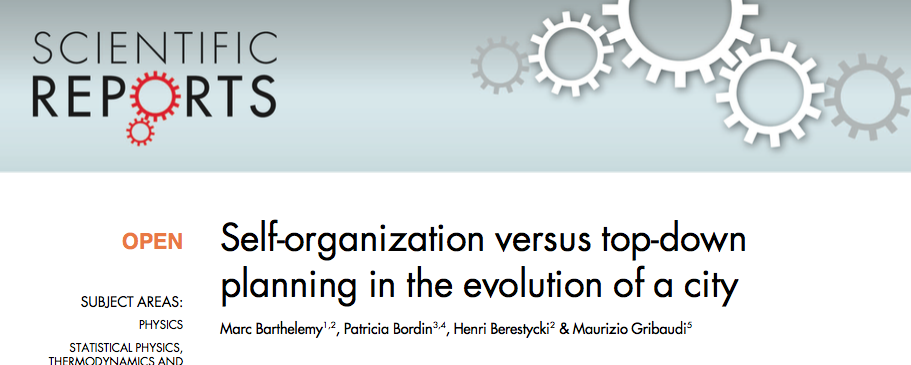
\includegraphics[width=\textwidth]{figures/bartpaper}

}
%%%%%%%%%%%%%%%%%


%%%%%%%%%%%%%%%%%
\sframe{But to what purpose ?}{

Exaggerating agent-based modeling ?

% Axtell economy
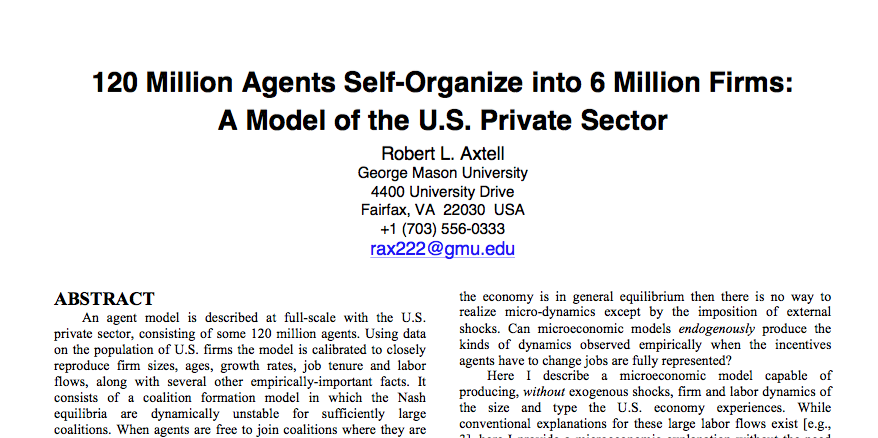
\includegraphics[width=\textwidth]{figures/exaxt}

}
%%%%%%%%%%%%%%%%%



%%%%%%%%%%%%%%%%%
\sframe{But to what purpose ?}{
% here trash Gibrat simulation ?

\textit{Other worrying examples :}

\begin{itemize}
\item Waste computational ressources to simulate mean and variance of Gibrat model ( = recheck the Central Limit Theorem !), which is fully solved otherwise~\cite{gabaix1999zipf}
\item Recently seen on Geotamtam : reach on new data (Pokemon Go) before thinking !
\end{itemize}

}
%%%%%%%%%%%%%%%%%








%%%%%%%%%%%%%%%%%
\sframe{Theories and Computation}{
% state the main idea
% -> Claims : make a stronger link between computational practices and maths/stats ? (if possible) - need more interdisciplinarity to do that.
%%     Geography in the center of that dynamic, but not all for granted ! (eg not simulate Gibrat as the fool example !)
%%     It implies the need for elaborated theory : here trash West/Bettencourt.

\textbf{Claim : } The computational shift~\cite{arthur2015complexity} and simulation practices will be central in geography~\cite{banos2013pour}, but are also dangerous :
\begin{itemize}
\item Data deluge may impose research subjects and elude theory
\item Computation may elude model construction and solving
\end{itemize}

\medskip

$\rightarrow$ \textit{Make a stronger link between computational practices, mathematics/statistics and theoretical geography} (Note : precise purpose of TQG, but seems forgotten sometimes)

$\rightarrow$ \textit{Theoretical and Quantitative Geography in the center of this dynamic}

}
%%%%%%%%%%%%%%%%%



%%%%%%%%%%%%%%%%%
\section{Case study}
%%%%%%%%%%%%%%%%%

% develop concrete example


\sframe{Case study : Context and Rationale}{
% interactions between networks and territories

\textbf{Study of interactions between network and territories :}

\medskip

$\rightarrow$ \textit{searching for stylized facts, what can be learnt from static correlations between urban form and road network ?}

\bigskip

\textbf{Theoretical Background : } \textit{A Theory of co-evolutive networked human territories} proposed in~\cite{raimbault2016memoire}, that in particular postulates an important role of networks in the morphogenesis of complex adaptive urban systems that are human territories


}


\sframe{Dataset construction}{
% brief description of nw simplification ; 

Computation of topological road network for all Europe, at 100m granularity scale (to be used consistently with population grid~\cite{eurostat})

\medskip

$\rightarrow$ Import of OSM into \texttt{pgsql}, simplification at 100m granularity, topological simplification with split/merge algorithm


\centering

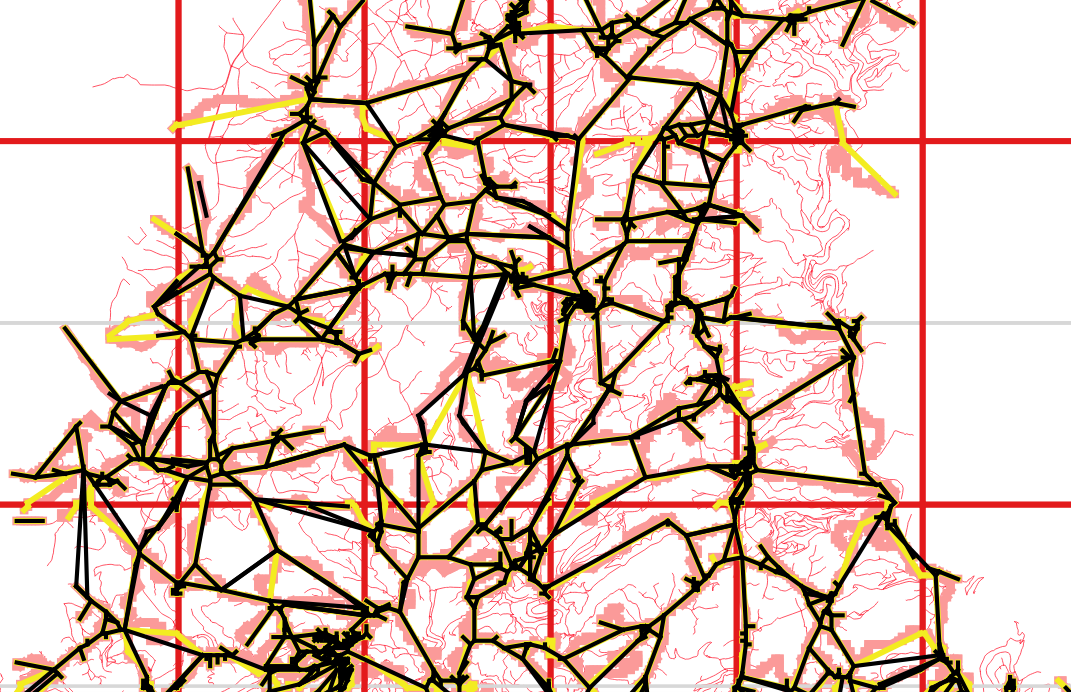
\includegraphics[width=0.6\textwidth]{figures/ex_nw}

}

\sframe{Locally stationary spatial correlations}{

$Y_i\left[\vec{x},t\right]$ spatio-temporal stochastic process, assumptions :
\begin{enumerate}
\item Local spatial autocorrelation is present and bounded by $l_{\rho}$ (in other words the processes are continuous in space) : at any $\vec{x}$ and $t$, $\left|\rho_{\norm{\Delta \vec{x}} < l_{\rho}}\left[Y_i (\vec{x}+\Delta \vec{x},t), Y_i (\vec{x},t) \right]\right| > 0$.
\item Processes are locally parametrized : $Y_i = Y_i\left[\alpha_i\right]$, where $\alpha_i (\vec{x})$ varies with $l_{\alpha}$, with $l_{\alpha} \gg l_{\rho}$.
\item Spatial correlations between processes have a sense at an intermediate scale $l$ such that $l_{\alpha}\gg l \gg l{\rho}$.
\item Processes covariance stationarity times scale as $\sqrt{l}$.
\item Local ergodicity is present at scale $l$ and dynamics are locally chaotic.
\end{enumerate}

}




%%%%%%%%%%%%%%%%%
\sframe{Stationarity and Ergodicity}{
Assuming local ergodicity, we have at least spatial and temporal local stationarities.

Spatial non-stationarity \textbf{at the second order}$\implies$ temporal scale variations $\implies$ non-ergodicity

}


%%%%%%%%%%%%%%%%%
\sframe{Results : Examples of indicators}{

% TODO : implementation ?

\textit{Computation of urban form indicators~\cite{le2015forme} and network indicators on 10km side square}

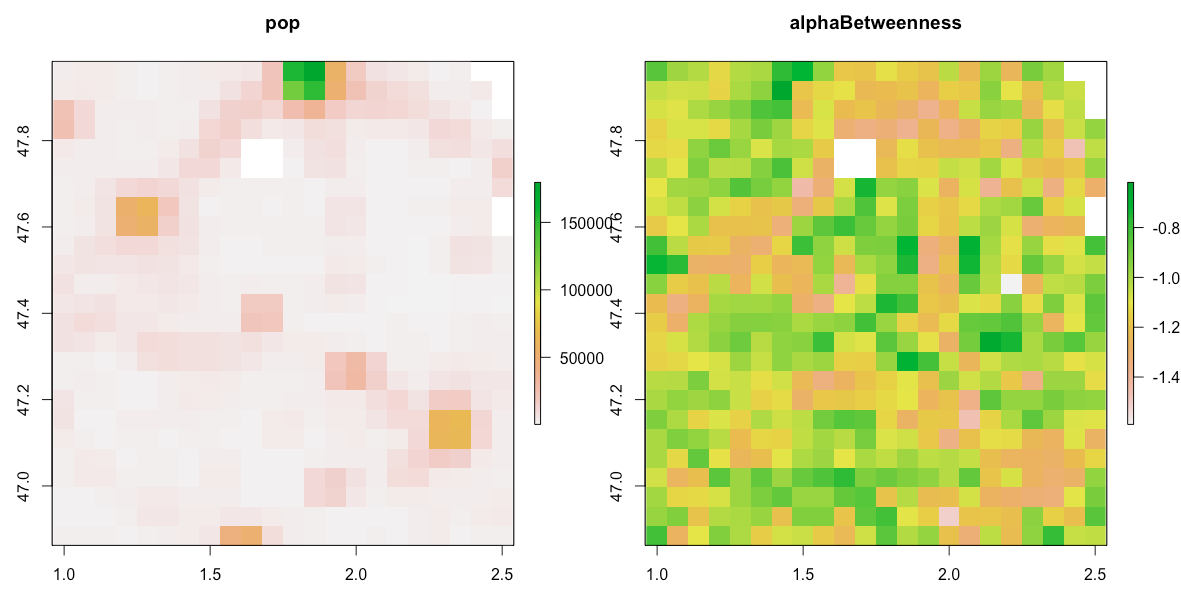
\includegraphics[width=\textwidth]{figures/pop-alphaBetweenness}

}


%%%%%%%%%%%%%%%%%
\sframe{Results : Examples of correlations}{

}


%%%%%%%%%%%%%%%%%
\sframe{Results : Stationarity scales}{
% maps

}



%%%%%%%%%%%%%%%%%
\sframe{Results : Stationarity scales}{
% plots

}



%%%%%%%%%%%%%%%%%
\sframe{Case study : implications}{
% thematic conclusion of the case study on ergodicity

$\rightarrow$ we show the regional nature of network-territories interactions, in particular the non-ergodicity of urban systems on these components

$\rightarrow$ no direct results on time dynamics, but still explorations to do : variable correlations areas


}




%%%%%%%%%%%%%%%%%
\section{Discussion}
%%%%%%%%%%%%%%%%%

% explain why example justify our point of view


%%%%%%%%%%%%%%%%%
\sframe{Discussion}{

1. \textit{Is a theory-free quantitative geography possible ?}

$\rightarrow$ close to the trap of black-box data-mining analysis ; still poor explanatory power, can exhibit relations but not reconstruct processes


\bigskip

2. \textit{Is a pure computational quantitative geography possible ?}

$\rightarrow$ even gaining 3 orders of magnitudes in computational power does not solve the dimensionality curse

\medskip

\textbf{In our case study : } 


}





%%%%%%%%%%%%%%%%%
\sframe{Conclusion}{

}



%%%%%%%%%%%%%%%%%
\sframe{Reserve}{

\textbf{Reserve Slides}

}
%%%%%%%%%%%%%%%%%%%%%%%%%%%%



%%%%%%%%%%%%%%%%%
\sframe{Network Simplification Algorithm}{

\begin{enumerate}
\item Filter OSM links (highway tag) and insert into \texttt{pgsql} with \texttt{osmosis} \cite{} % TODO
\item First simplification : two cells of base raster (population density) are linked if and only if they are linked by OSM link (associated type/speed)
\item Topological simplification :
\begin{itemize}
\item split the space into a partition, simplify within each box
\item construct independent merging subsets of the partition, merge sequentially for each subset.
\end{itemize}

\end{enumerate}

$\rightarrow$
% TODO summary stats etc

}
%%%%%%%%%%%%%%%%%%%%%%%%%%%%


%%%%%%%%%%%%%%%%%
\sframe{Indicators}{

\textbf{Morphological Indicators : } Density, Spatial Autocorrelation, Entropy, Mean Distance, Hierarchy

\bigskip

\textbf{Network Indicators : } betweenness (mean/hierarchy), closeness (mean/hierarchy), mean link length, network performance, mean path length, diameter, components, clustering coefficient, density

\bigskip

\textbf{Correlation Measures : } Pearson test ; correlation matrices then aggregated (mean, mean absolute, first principal component - % TODO
\% variance with $\delta = $)


}
%%%%%%%%%%%%%%%%%%%%%%%%%%%%



%%%%%%%%%%%%%%%%%%%%%%%%%%%%
\sframe{Theory : Pillars}{
\begin{enumerate}
\item \textit{Networked Human Territories} $\rightarrow$ Raffestin approach to territory combined with Dupuy theory of networks.
\item \textit{Evolutive Urban Theory} $\rightarrow$ City Systems as complex Adaptive systems, applied to human settlements in general and thus territorial systems.
\item \textit{Urban Morphogenesis} $\rightarrow$ Morphogenesis as autonomous rules to explain growth of urban form. Used as the provider of modular decompositions.
\item \textit{Boundaries and Co-evolution} $\rightarrow$ Co-evolution as the existence of \textit{niche}, consequence of boundary patterns.
\end{enumerate}
}
%%%%%%%%%%%%%%%%%%%%%%%%%%%%

%%%%%%%%%%%%%%%%%%%%%%%%%%%%
\sframe{Theory : Specification}{
\begin{itemize}
\jitem{Previous def. of territorial systems}
\jitem{Modular decomposition and stationarity : existence of scales}
\jitem{Feedback loops between and inside scales yield weak emergence, thus complexity}
\jitem{Morphogenesis gives modular decomposition and co-evolution}
\jitem{\textbf{Main assumption.} Necessity of Networks : networks are necessary component of co-evolutive niches.}
\end{itemize}
}
%%%%%%%%%%%%%%%%%%%%%%%%%%%%




%%%%%%%%%%%%%%%%%%%%%
\begin{frame}[allowframebreaks]
\frametitle{References}
\bibliographystyle{apalike}
\bibliography{/Users/Juste/Documents/ComplexSystems/CityNetwork/Biblio/Bibtex/CityNetwork}
\end{frame}
%%%%%%%%%%%%%%%%%%%%%%%%%%%%












\end{document}















